\documentclass[conference,a4paper]{IEEEtran}
\IEEEoverridecommandlockouts
\usepackage[utf8]{inputenc}
\usepackage[T1]{fontenc}
\usepackage[spanish,es-noshorthands,es-tabla]{babel}
\usepackage{cite}
\usepackage{amsmath,amssymb}
\usepackage{graphicx}
\usepackage{booktabs}
\usepackage{multirow}
\usepackage{xcolor}
\usepackage{tikz}
\usetikzlibrary{arrows.meta,positioning,fit,backgrounds}
\usepackage[hidelinks]{hyperref}
\usepackage{xurl}
\graphicspath{{figures/}{../docs/figures/}}
\renewcommand{\IEEEkeywordsname}{Palabras clave}
\def\BibTeX{{\rm B\kern-.05em{\sc i\kern-.025em b}\kern-.08em T\kern-.1667em\lower.7ex\hbox{E}\kern-.125emX}}

\begin{document}

\title{Analítica de datos para la detección de cojera equina: minería del estado del arte, perfilamiento de datasets y señales de marcha en una arquitectura en la nube\\
\large Avance del proyecto integrador (Minería de Datos, Machine Learning y Cloud Computing)}

\author{\IEEEauthorblockN{Carlos Josué Barrera Vargas}
\IEEEauthorblockA{Facultad de Ingeniería de Datos e Inteligencia Artificial\\
Universidad Santo Tomás, Seccional Tunja, Colombia\\
Quinto semestre · Segundo periodo de 2026}}

\maketitle

\begin{abstract}
La cojera es el problema de salud más frecuente y costoso en los equinos, y su diagnóstico visual tiene baja concordancia entre veterinarios cuando la cojera es leve. Este avance presenta la fase exploratoria de un sistema de apoyo a la detección temprana de cojera que, en su versión final, usará visión por computador. Siguiendo CRISP-DM, se integran tres fuentes: (i) un corpus de 4.024 artículos obtenidos por \emph{web scraping} de la API de OpenAlex, analizado con EDA, detección de outliers, clustering de texto (TF-IDF, SVD y K-Means) y reglas de asociación (FP-Growth); (ii) un catálogo de 14 datasets públicos, perfilados con distancia de Gower y clustering jerárquico; y (iii) un dataset abierto de sensores inerciales de 22 caballos con cojera inducida, del que se extrajeron 1.817 zancadas con 27 métricas de simetría. Las métricas reproducen la biomecánica conocida: la asimetría vertical de la cabeza casi se duplica en cojera anterior y la del sacro aumenta un 53\,\% en cojera posterior (Wilcoxon, $p<0{,}05$). Un Random Forest optimizado por Grid Search y validado por caballo alcanza un ROC-AUC de 0,71 con caballos no vistos, interpretado con SHAP. El análisis muestra que ningún dataset público combina video de caballos con etiqueta de cojera, y que solo 1 de 175 trabajos sobre caballo, cojera y visión tiene autores en Colombia. Se propone una arquitectura serverless en AWS desplegada con Terraform, con un costo estimado menor de USD 0,40 al mes en el escenario académico (USD 0,13 con la capa gratuita). El proyecto contribuye a los ODS 3 y 8.
\end{abstract}

\begin{IEEEkeywords}
minería de datos, CRISP-DM, cojera equina, clustering, reglas de asociación, aprendizaje automático, computación en la nube, objetivos de desarrollo sostenible
\end{IEEEkeywords}

% =====================================================================
\section{Introducción}
Colombia es uno de los países con mayor población equina de América. El censo del ICA de 2025 reportó 964.426 equinos~\cite{agronegocios2025censo}, y el caballo criollo de paso tiene un peso cultural y económico importante, especialmente en regiones ganaderas como Boyacá. En el mundo, la cojera es el problema veterinario más frecuente de los caballos: en la primera encuesta nacional de salud equina del Reino Unido, casi el 19\,\% de los animales tenía cojera, principalmente por enfermedad articular degenerativa~\cite{nehs2013}. En Estados Unidos, el estudio NAHMS \emph{Equine'98} la clasificó como la condición más costosa entre las evaluadas, por su alta incidencia, los días de uso perdidos y los gastos veterinarios~\cite{usda1998}.

El diagnóstico se basa sobre todo en la observación del caballo al trote. Sin embargo, la evaluación subjetiva es poco fiable cuando la cojera es leve. Keegan \emph{et al.}~\cite{keegan2010} encontraron que, tras un examen completo, los clínicos coincidían en si un miembro estaba cojo solo el 72,9\,\% de las veces ($\kappa=0{,}45$). En evaluaciones en círculo a partir de video, la concordancia entre veterinarios bajó a $\kappa=0{,}31$, y fue aún menor para la cojera posterior~\cite{hammarberg2016}. Esto motiva sistemas objetivos de bajo costo, en particular los basados en video de un teléfono móvil, que no requieren instrumentar al animal.

Este documento presenta el \textbf{avance} del proyecto integrador. Antes de entrenar un modelo de visión, se usa minería de datos para responder tres preguntas: \emph{¿qué se ha investigado y dónde está el vacío?}, \emph{¿con qué datos públicos se puede construir el sistema?} y \emph{¿qué señales de la marcha distinguen a un caballo cojo?} Las contribuciones son: (1) un pipeline reproducible de adquisición y preparación desde una API, un catálogo curado y señales crudas de sensores; (2) perfiles e interpretación de outliers en las tres fuentes; (3) un modelo preliminar interpretable validado con caballos no vistos; y (4) una arquitectura cloud como código, con su estimación de costos.

% =====================================================================
\section{Planteamiento del problema y alineación con los ODS}
\subsection{Problema}
La detección temprana de cojera depende de la observación experta, que es subjetiva, varía entre evaluadores y no está al alcance de muchos criadores y propietarios rurales. Los sistemas objetivos existentes (sensores inerciales, plataformas de fuerza, captura de movimiento) son costosos o requieren instrumentar al animal. La visión por computador puede cerrar esa brecha, pero exige datos etiquetados y validación clínica.

\textbf{Pregunta del proyecto:} ¿es posible estimar, a partir de datos de movimiento obtenibles con tecnología accesible, la probabilidad de que un caballo presente cojera, de forma interpretable y desplegable a bajo costo?

\textbf{Usuarios y beneficiarios:} veterinarios de campo (segunda opinión objetiva y seguimiento), criadores y asociaciones de caballo criollo (vigilancia rutinaria) y, en última instancia, los animales (diagnóstico más temprano).

\subsection{Alineación con los ODS}
\textbf{ODS 3 (salud y bienestar)}, bajo el enfoque \emph{Una Salud}, que integra la salud animal y humana~\cite{un2015}: la detección temprana reduce el dolor y la progresión de lesiones articulares. \textbf{ODS 8 (trabajo decente y crecimiento económico)}: menos días de uso perdidos y menores costos para un sector rural intensivo en empleo.

\subsection{Objetivos de este avance}
(1) Construir y limpiar un corpus del estado del arte mediante una API (web scraping). (2) Perfilar líneas de investigación, interpretar outliers y descubrir asociaciones entre conceptos. (3) Perfilar los datasets públicos disponibles. (4) Validar con datos reales qué métricas de marcha distinguen la cojera y entrenar un modelo preliminar. (5) Diseñar la arquitectura en la nube, implementarla como código y estimar sus costos.

% =====================================================================
\section{Trabajo relacionado}
La evaluación objetiva de la cojera equina se ha basado en sensores inerciales colocados en cabeza y pelvis, que miden la asimetría del desplazamiento vertical (MinDiff, MaxDiff). Estas medidas se correlacionan con el examen subjetivo, aunque la concordancia es solo de leve a moderada~\cite{keegan2013}. En visión por computador, la estimación de pose sin marcadores con DeepLabCut~\cite{mathis2018} impulsó benchmarks específicos: Horse-10 (30 caballos, 22 puntos anatómicos, 8.114 frames) evalúa la generalización a caballos no vistos~\cite{mathis2021}, y PFERD ofrece video multivista sincronizado con captura 3D de más de 100 marcadores en cinco caballos~\cite{li2024pferd}. Los benchmarks multiespecie AP-10K (10.015 imágenes de 54 especies)~\cite{yu2021ap10k}, APT-36K (2.400 clips de video de 30 especies)~\cite{yang2022apt36k} y Animal Kingdom (33 mil frames de 850 especies)~\cite{ng2022animalkingdom} amplían la escala, pero no incluyen etiquetas clínicas. La detección automática de cojera está más avanzada en bovinos, con bases públicas como CowScreeningDB (sensores de 43 vacas)~\cite{ismail2024cow}. El análisis de este avance (sección~\ref{sec:resultados}) cuantifica ese desequilibrio y la ausencia de datos abiertos que combinen video equino y cojera.

% =====================================================================
\section{Sistema propuesto}
La Fig.~\ref{fig:sistema} resume el sistema completo. Una capa de adquisición alimenta un data lake. El pipeline KDD/CRISP-DM produce datasets limpios y perfiles. El modelo de ML se entrena con métricas de simetría y se sirve por una API. En la fase final, el bloque de visión estimará esas mismas métricas desde video mediante keypoints de cabeza, cruz y pelvis, de modo que el clasificador de este avance se reutiliza.

\begin{figure}[t]
\centering
\begin{tikzpicture}[node distance=3mm and 4mm, font=\scriptsize,
  b/.style={draw, rounded corners=2pt, align=center, minimum height=7mm, text width=17mm, fill=#1!12},
  b/.default=blue, >={Stealth[length=1.6mm]}]
\node[b=orange] (api) {API OpenAlex\\(scraping)};
\node[b=orange, below=of api] (cat) {Catálogo de\\datasets};
\node[b=orange, below=of cat] (imu) {Dataverse\\(IMU 500 Hz)};
\node[b=gray, below=of imu] (vid) {Video móvil\\(fase final)};
\node[b=green, right=6mm of cat, yshift=-5mm, text width=14mm, minimum height=22mm] (lake) {Data lake S3\\raw / processed / models};
\node[b, right=6mm of lake, yshift=10mm] (kdd) {KDD / CRISP-DM\\limpieza, EDA,\\PCA, clustering,\\reglas};
\node[b, below=of kdd] (ml) {ML: ensemble +\\Grid Search +\\SHAP};
\node[b=gray, below=of ml] (cv) {Visión: keypoints\\$\rightarrow$ métricas de\\simetría};
\node[b=purple, right=4mm of ml, text width=13mm] (srv) {API REST\\(Lambda)\\+ DynamoDB};
\draw[->] (api) -- (lake); \draw[->] (cat) -- (lake); \draw[->] (imu) -- (lake);
\draw[->, dashed] (vid.east) -- ++(2mm,0) |- (cv.west);
\draw[->] (lake) -- (kdd); \draw[->] (kdd) -- (ml); \draw[->, dashed] (cv) -- (ml); \draw[->] (ml) -- (srv);
\begin{scope}[on background layer]
\node[draw=gray, dashed, rounded corners, fit=(api)(vid), inner sep=2pt, label={[font=\tiny]above:Adquisición}] {};
\end{scope}
\end{tikzpicture}
\caption{Diagrama de bloques del sistema. En gris, los componentes de la fase de visión por computador (entrega final).}
\label{fig:sistema}
\end{figure}

% =====================================================================
\section{Pipeline de minería de datos (CRISP-DM)}
\label{sec:mineria}
El proceso sigue las fases de CRISP-DM~\cite{wirth2000}: comprensión del negocio y de los datos, preparación, modelado y evaluación.
\subsection{Adquisición}
\textbf{Fuente 1, corpus científico (web scraping):} cliente en Python para la API REST de OpenAlex~\cite{priem2022openalex}, con paginación por cursor, reintentos exponenciales y clave de API guardada fuera del código. Usa cinco consultas booleanas sobre título y resumen (cojera equina, marcha equina, sensores inerciales, visión y pose animal, y cojera con ML en otras especies), con los 1.500 registros más relevantes de cada una, para un total de 6.472 registros crudos. El mismo código se despliega como función Lambda semanal (sección~\ref{sec:cloud}).

\textbf{Fuente 2, catálogo de datasets:} 14 datasets identificados en la revisión, con 18 atributos (modalidad, especie, tamaño, keypoints, etiquetas, licencia, acceso) y la URL de su fuente. Los atributos que la fuente no reporta se dejan como faltantes en lugar de estimarlos.

\textbf{Fuente 3, señales IMU:} dataset abierto de Smit \emph{et al.}~\cite{smit2023dataset} (CC BY 4.0): 22 caballos islandeses (10 con cojera anterior y 12 con cojera posterior inducida), medidos antes (BAS) y durante (IND) la inducción con 16 sensores a 500 Hz. Se descargaron por la API de Dataverse las pruebas de caballo llevado a mano (86 archivos, 6,2 GB, en formatos MATLAB v5 y v7.3/HDF5).

\subsection{Preparación y transformación}
\textbf{Corpus:} se fusionaron duplicados entre consultas, conservando el número de consultas como variable de interdisciplinariedad. Se excluyeron tipos no científicos (informes de revisión, erratas) y un trabajo retractado, se restringió la ventana a 1990--2026, se eliminaron duplicados preprint/versión publicada por título normalizado y se aplicó un filtro de pertinencia temática. Las reglas de asociación revelaron ruido residual (estudios de cinemática espermática), que también se excluyó. Resultado: \textbf{4.024 artículos} (Tabla~\ref{tab:limpieza}). Tratamiento de nulos: país desconocido como categoría propia (24\,\%); resumen faltante marcado con una bandera, usando título y palabras clave como texto; el FWCI no se imputa, para no inventar impacto.

\begin{table}[t]
\centering
\caption{Trazabilidad de la limpieza del corpus}
\label{tab:limpieza}
\begin{tabular}{lr}
\toprule
Paso & Registros \\
\midrule
Registros crudos (5 consultas) & 6.472 \\
Únicos por identificador & 5.862 \\
Sin tipos no científicos ni retractados & 5.430 \\
Ventana 1990--2026 & 5.166 \\
Sin duplicados por título & 4.995 \\
Filtro de pertinencia temática & \textbf{4.024} \\
\bottomrule
\end{tabular}
\end{table}

\textbf{Señales IMU (ingeniería de características):} en cada segmento de trote en línea recta, la aceleración de cabeza, cruz, sacro y tuberosidades coxales se proyectó sobre la dirección media de la gravedad, se filtró (Butterworth 0,3--20 Hz), se decimó a 100 Hz y se integró dos veces con filtros paso alto para obtener el desplazamiento vertical. Las zancadas se segmentaron con los máximos del sacro (periodo estimado por autocorrelación). Por zancada se calcularon: MinDiff, MaxDiff y rango de movimiento (ROM) en mm; \emph{harmonic ratio} y RMS de la aceleración vertical; diferencia de ROM entre tuberosidades coxales (\emph{hip hike}); y duración. Así, unos 50 millones de muestras se reducen a \textbf{1.835 zancadas $\times$ 27 variables} con significado clínico. Los nulos de la cruz (2,3\,\%, un archivo sin ese sensor) se imputaron de forma jerárquica (mediana del caballo y la condición; si no existe, del experimento y la condición). Se eliminaron 18 zancadas físicamente imposibles (1\,\%), por duración fuera de 0,45--0,85 s o ROM mayor de 200 mm.

\subsection{Detección e interpretación de outliers}
En el corpus, el impacto ajustado por antigüedad (citas por año) tiene asimetría de 37. Se combinaron IQR sobre $\log(1+x)$ y z-score robusto con MAD ($|z|>3{,}5$)~\cite{iglewicz1993}, que marcaron 87 trabajos atípicos. No se eliminaron: el 77\,\% de ellos usa visión por computador (frente al 32\,\% del resto), tienen el doble de autores y el 88\,\% está en acceso abierto. Son las herramientas fundacionales (DeepLabCut, SLEAP, DeepPoseKit), es decir, la frontera tecnológica del área. En el IMU, Isolation Forest (5\,\%) encontró casi el doble de anomalías en la cojera posterior inducida (7,3\,\% frente a 4,1\,\%), con asimetrías mayores: la anomalía es en buena parte la señal clínica. Un solo caballo concentra el 25\,\% de las anomalías, un perfil individual atípico que se vigila en la validación.

\subsection{Minería no supervisada}
\textbf{Clustering de texto:} TF-IDF (unigramas y bigramas, 14.897 términos) reducido con TruncatedSVD a 100 componentes y normalizado (equivalente a la similitud coseno). K-Means se evaluó para $k=3$--14 con codo, silhouette, Calinski-Harabasz y Davies-Bouldin. Se eligió $k=8$ por su equilibrio entre métricas e interpretabilidad. Ward produjo agrupaciones parcialmente concordantes (ARI = 0,35). DBSCAN se descartó: dejó el 47\,\% de los artículos como ruido, el caso típico de densidades homogéneas en alta dimensión.

\textbf{Reglas de asociación:} cada artículo es una transacción con sus palabras clave (las 150 más frecuentes). Apriori y FP-Growth produjeron los mismos 222 conjuntos frecuentes (soporte $\geq 0{,}008$); FP-Growth fue más rápido. Se retuvieron 52 reglas con lift $\geq 1{,}5$ y confianza $\geq 0{,}3$.

\textbf{IMU y catálogo:} PCA sobre las 27 métricas estandarizadas (15 componentes explican el 90\,\%), K-Means sobre esos componentes, clustering jerárquico de perfiles caballo-condición y, para el catálogo, distancia de Gower con enlace promedio, que mezcla variables binarias, ordinales y numéricas con faltantes.

% =====================================================================
\section{Modelo de machine learning (preliminar)}
\label{sec:ml}
\textbf{Tarea:} clasificar cada zancada como sana (BAS) o coja (IND). \textbf{Decisión clave:} las zancadas de un mismo caballo no son independientes, así que toda la validación se \emph{agrupa por caballo}. Se reservaron 5 caballos completos como prueba (de ambos experimentos y con clases balanceadas). La selección de modelos y la optimización usan GroupKFold (5) sobre los 17 restantes, y la robustez se mide con \emph{Leave-One-Horse-Out} (LOHO) sobre los 22.

\textbf{Pipeline:} imputación por mediana, estandarización y modelo, ajustados dentro de cada fold para evitar fugas de información. Modelos base: regresión logística, KNN y SVM (RBF). Ensembles: Random Forest, AdaBoost y Gradient Boosting. Optimización: Grid Search para Random Forest (36 combinaciones de profundidad, hojas mínimas, número de árboles y variables por división) y Gradient Boosting (16), y Random Search (30 iteraciones, distribución log-uniforme) para SVM. Métrica principal: ROC-AUC. Interpretabilidad: TreeSHAP~\cite{lundberg2017} e importancia por permutación.

% =====================================================================
\section{Arquitectura en la nube}
\label{sec:cloud}
Se eligió \textbf{AWS, nube pública} con un diseño \textbf{serverless} (Fig.~\ref{fig:aws}), porque la carga es intermitente: una ingesta semanal y predicciones esporádicas. Con este diseño se paga solo por uso, sin servidores ociosos.
\begin{itemize}
\item \textbf{Ingesta (FaaS):} EventBridge programa una Lambda en Graviton (arm64, más barata por GB-s) que ejecuta el scraping y escribe JSON crudo en S3. La clave de API se guarda cifrada en SSM Parameter Store (nivel estándar, sin costo).
\item \textbf{Almacenamiento:} data lake en S3 con zonas \texttt{raw/}, \texttt{processed/} y \texttt{models/}, cifrado, versionado, con acceso público bloqueado y ciclo de vida que pasa los datos crudos a Glacier a los 90 días.
\item \textbf{Analítica (PaaS):} Glue Data Catalog y Athena para consultar con SQL sobre S3, con un límite de 1 GB escaneado por consulta para controlar costos.
\item \textbf{Base de datos:} DynamoDB \emph{on-demand} para el registro de predicciones por caballo, con recuperación a un punto en el tiempo (PITR).
\item \textbf{Inferencia (FaaS + API):} API Gateway HTTP con \emph{throttling} y una Lambda con imagen Docker (scikit-learn) en ECR que carga el modelo desde S3.
\item \textbf{Escalabilidad y alta disponibilidad:} Lambda, API Gateway, S3 y DynamoDB escalan automáticamente y operan en varias zonas de disponibilidad de forma gestionada, así que no requieren balanceadores ni grupos de autoescalado.
\item \textbf{Recuperación ante desastres:} versionado de S3, PITR de 35 días en DynamoDB y replicación opcional entre regiones (us-west-2, Standard-IA). Los objetivos son RPO en minutos y RTO menor de una hora, ya que la infraestructura completa se recrea con \texttt{terraform apply}.
\item \textbf{Operación:} CloudWatch con alarma de errores, SNS y un presupuesto mensual con alertas al 80\,\% y 100\,\%.
\end{itemize}
Todo está escrito en \textbf{Terraform} (8 archivos, proveedor AWS 5.x, 38 bloques de recursos, con mínimo privilegio en IAM y etiquetas para atribuir costos). Se validó con \texttt{terraform validate} y la API de inferencia se activa con una variable.

\begin{figure}[t]
\centering
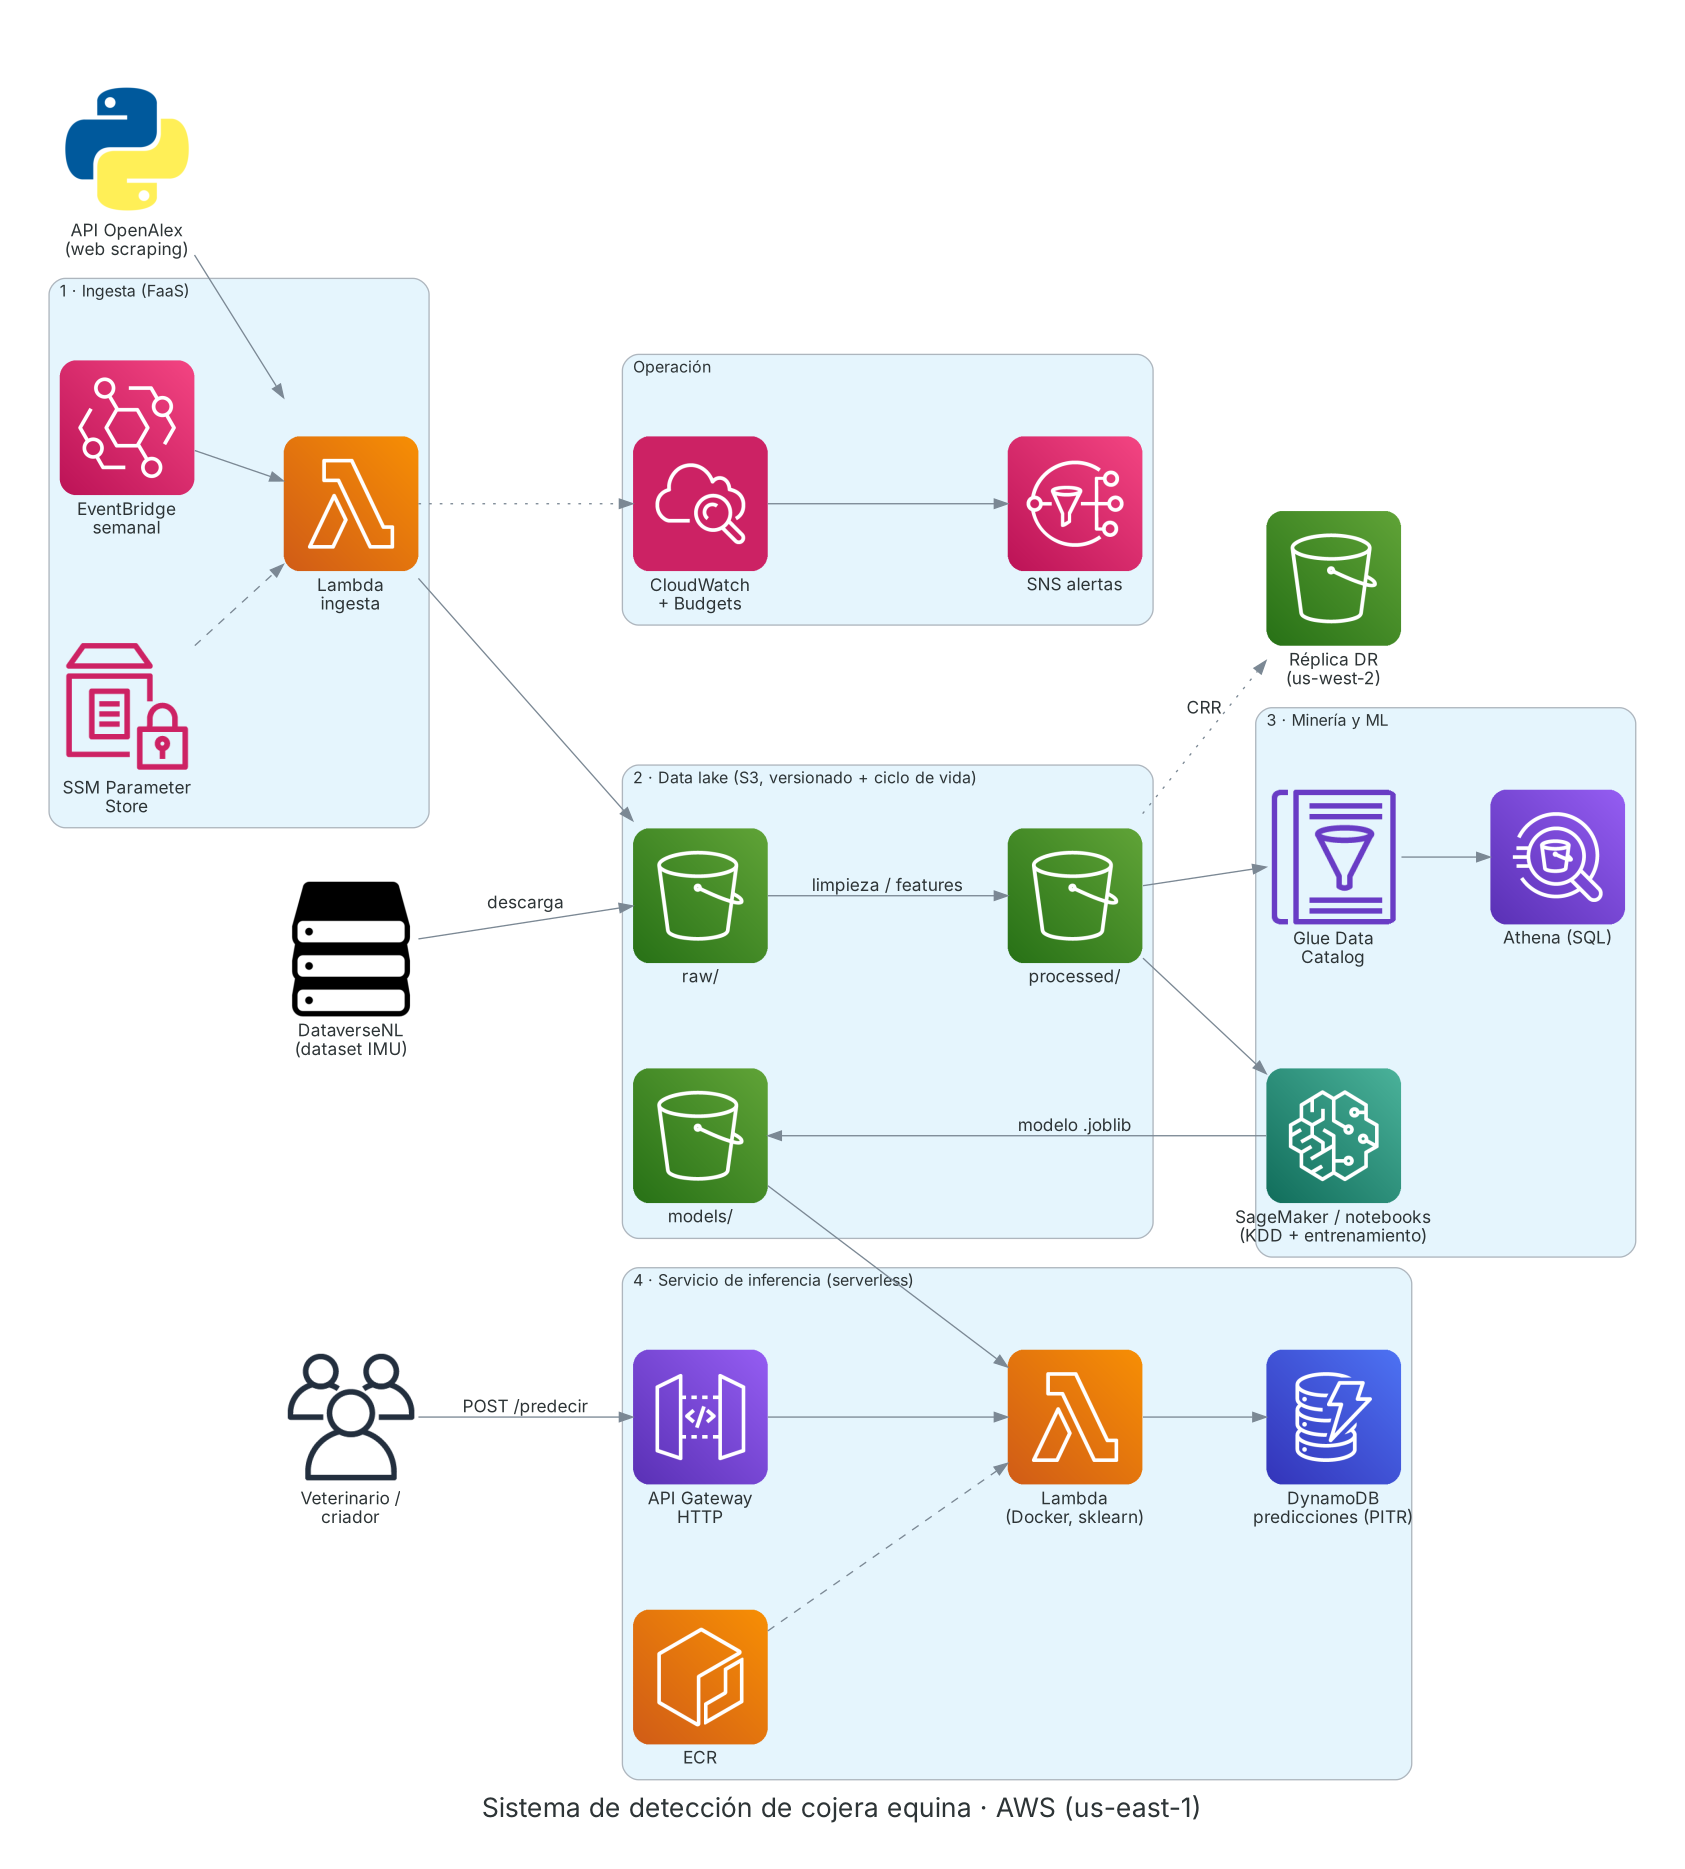
\includegraphics[width=\columnwidth]{arquitectura_aws.png}
\caption{Arquitectura en AWS. Los bloques 1, 2 y 4 y la operación están implementados en Terraform; SageMaker se incorporará en la fase final.}
\label{fig:aws}
\end{figure}

% =====================================================================
\section{Resultados preliminares}
\label{sec:resultados}
\subsection{Estado del arte: tendencias, perfiles y vacío}
La producción crece de forma sostenida, y desde 2020 los trabajos con visión por computador pasan del 21\,\% al 52\,\% del total, mientras los enfoques clínicos bajan del 47\,\% (1990--2005) al 30\,\% (2021--2026) (Fig.~\ref{fig:tendencia}). Estados Unidos, Reino Unido y China lideran; Latinoamérica tiene una presencia marginal. Los 8 perfiles (Tabla~\ref{tab:perfiles}) separan el bloque clínico veterinario (diagnóstico, patologías y cinemática, más antiguo y con menor impacto anual) del bloque tecnológico (pose, visión, sensores y bovinos, más reciente y con más outliers de impacto) (Fig.~\ref{fig:tsne}). Las reglas confirman la estructura del campo: \{cojera anterior + cojera equina\} $\rightarrow$ \{cojera posterior\} (lift = 16,0); \{estimación de pose humana\} $\rightarrow$ \{estimación de pose animal\} (lift = 22,8), que refleja la transferencia de métodos; y \{detección de cojera\} $\leftrightarrow$ \{ganado lechero\} (lift = 5,5), que indica que la \emph{detección automática} de cojera se ha desarrollado sobre todo en bovinos. \textbf{El vacío:} de 1.331 trabajos sobre caballo y cojera, solo 175 usan visión por computador, 5 tienen autores latinoamericanos y 1 tiene autores en Colombia.

\begin{figure}[t]
\centering
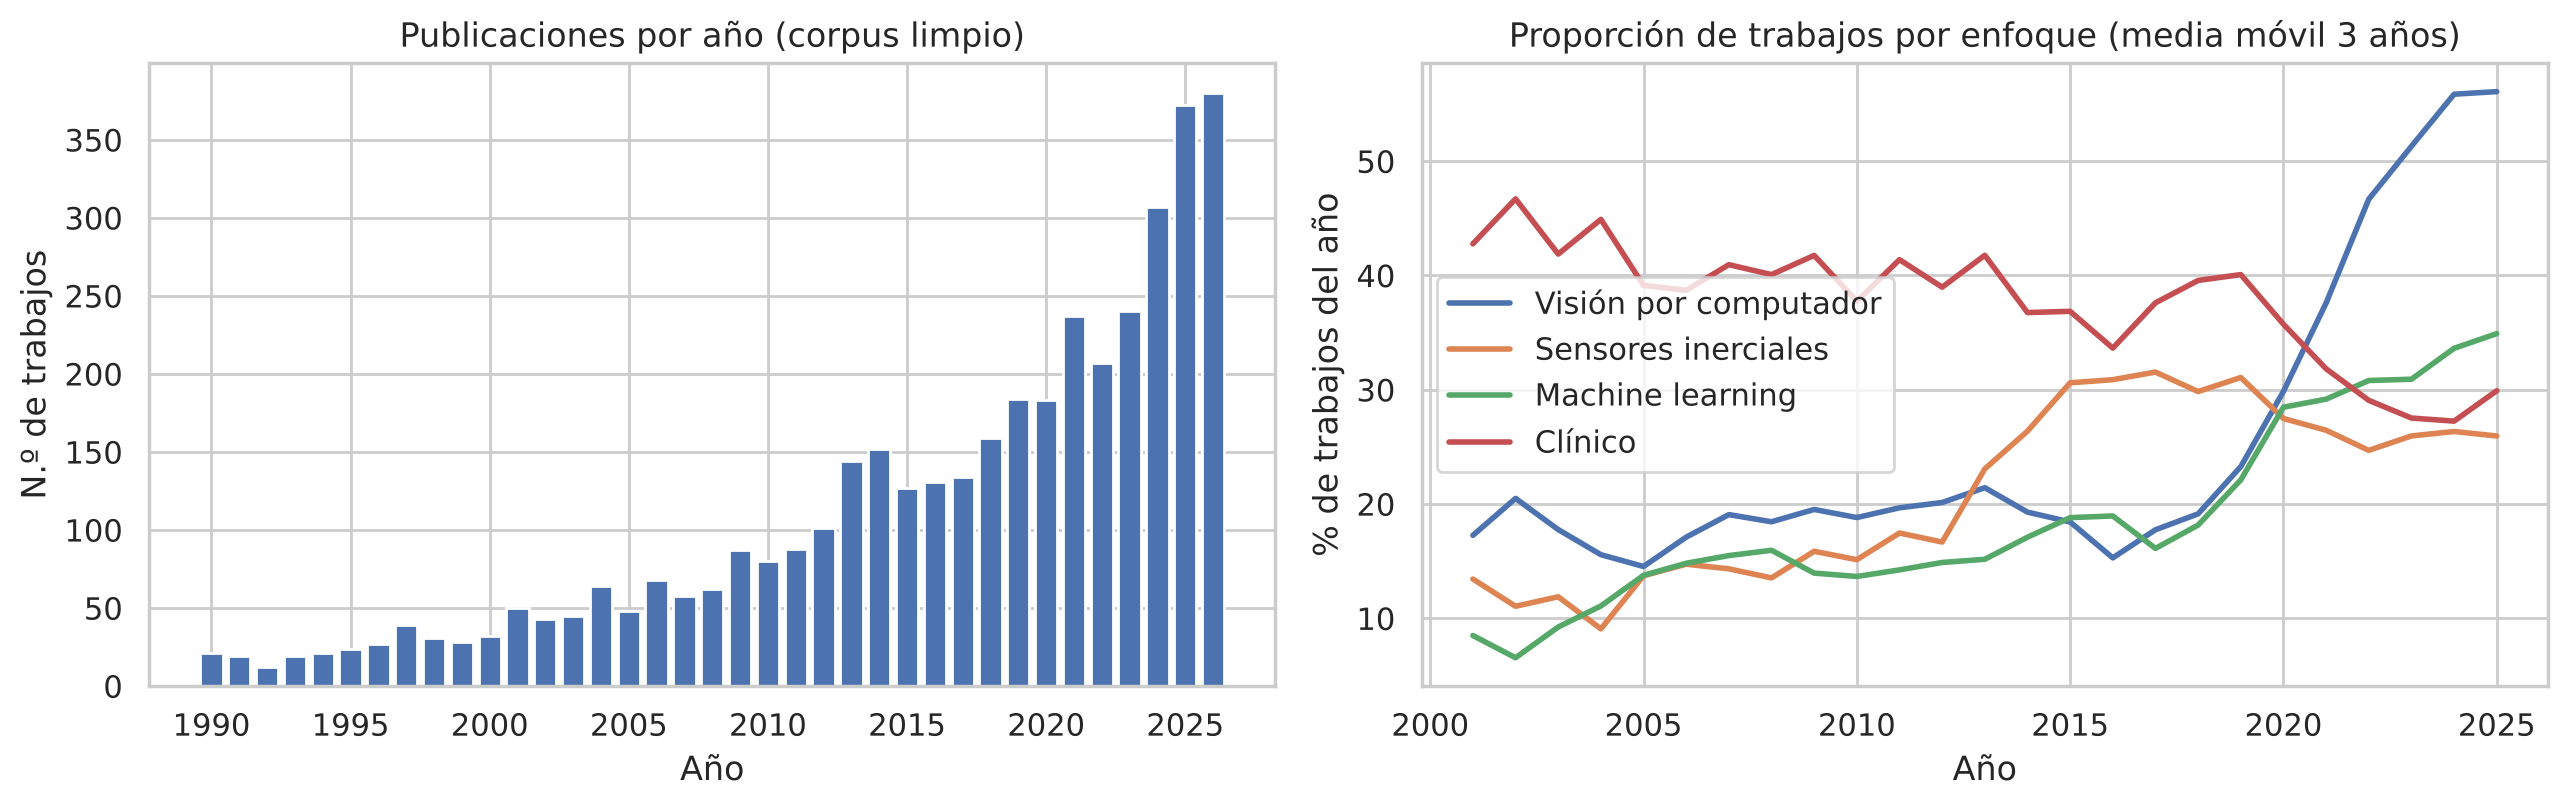
\includegraphics[width=\columnwidth]{art_tendencia_anual.png}
\caption{Publicaciones por año y proporción por enfoque (media móvil de 3 años). El año 2026 está incompleto (extracción en noviembre).}
\label{fig:tendencia}
\end{figure}

\begin{table}[t]
\centering
\caption{Perfiles de investigación (K-Means, $k=8$, 3.823 artículos en inglés)}
\label{tab:perfiles}
\footnotesize\setlength{\tabcolsep}{3pt}
\begin{tabular}{lrrr}
\toprule
Perfil & $n$ & Año med. & Citas/año med. \\
\midrule
Cinemática y biomecánica de la marcha & 755 & 2013 & 0,53 \\
Diagnóstico clínico de la cojera & 611 & 2016 & 0,53 \\
Genética, bienestar y rendimiento & 609 & 2020 & 0,33 \\
Patologías articulares y tratamiento & 476 & 2014 & 0,47 \\
Estimación de pose animal (deep learning) & 391 & 2024 & 1,00 \\
Sensores inerciales y asimetría & 364 & 2020 & 1,17 \\
Visión por computador (monitoreo animal) & 355 & 2024 & 0,71 \\
Detección de cojera en bovinos & 262 & 2022 & 2,00 \\
\bottomrule
\end{tabular}
\end{table}

\begin{figure}[t]
\centering
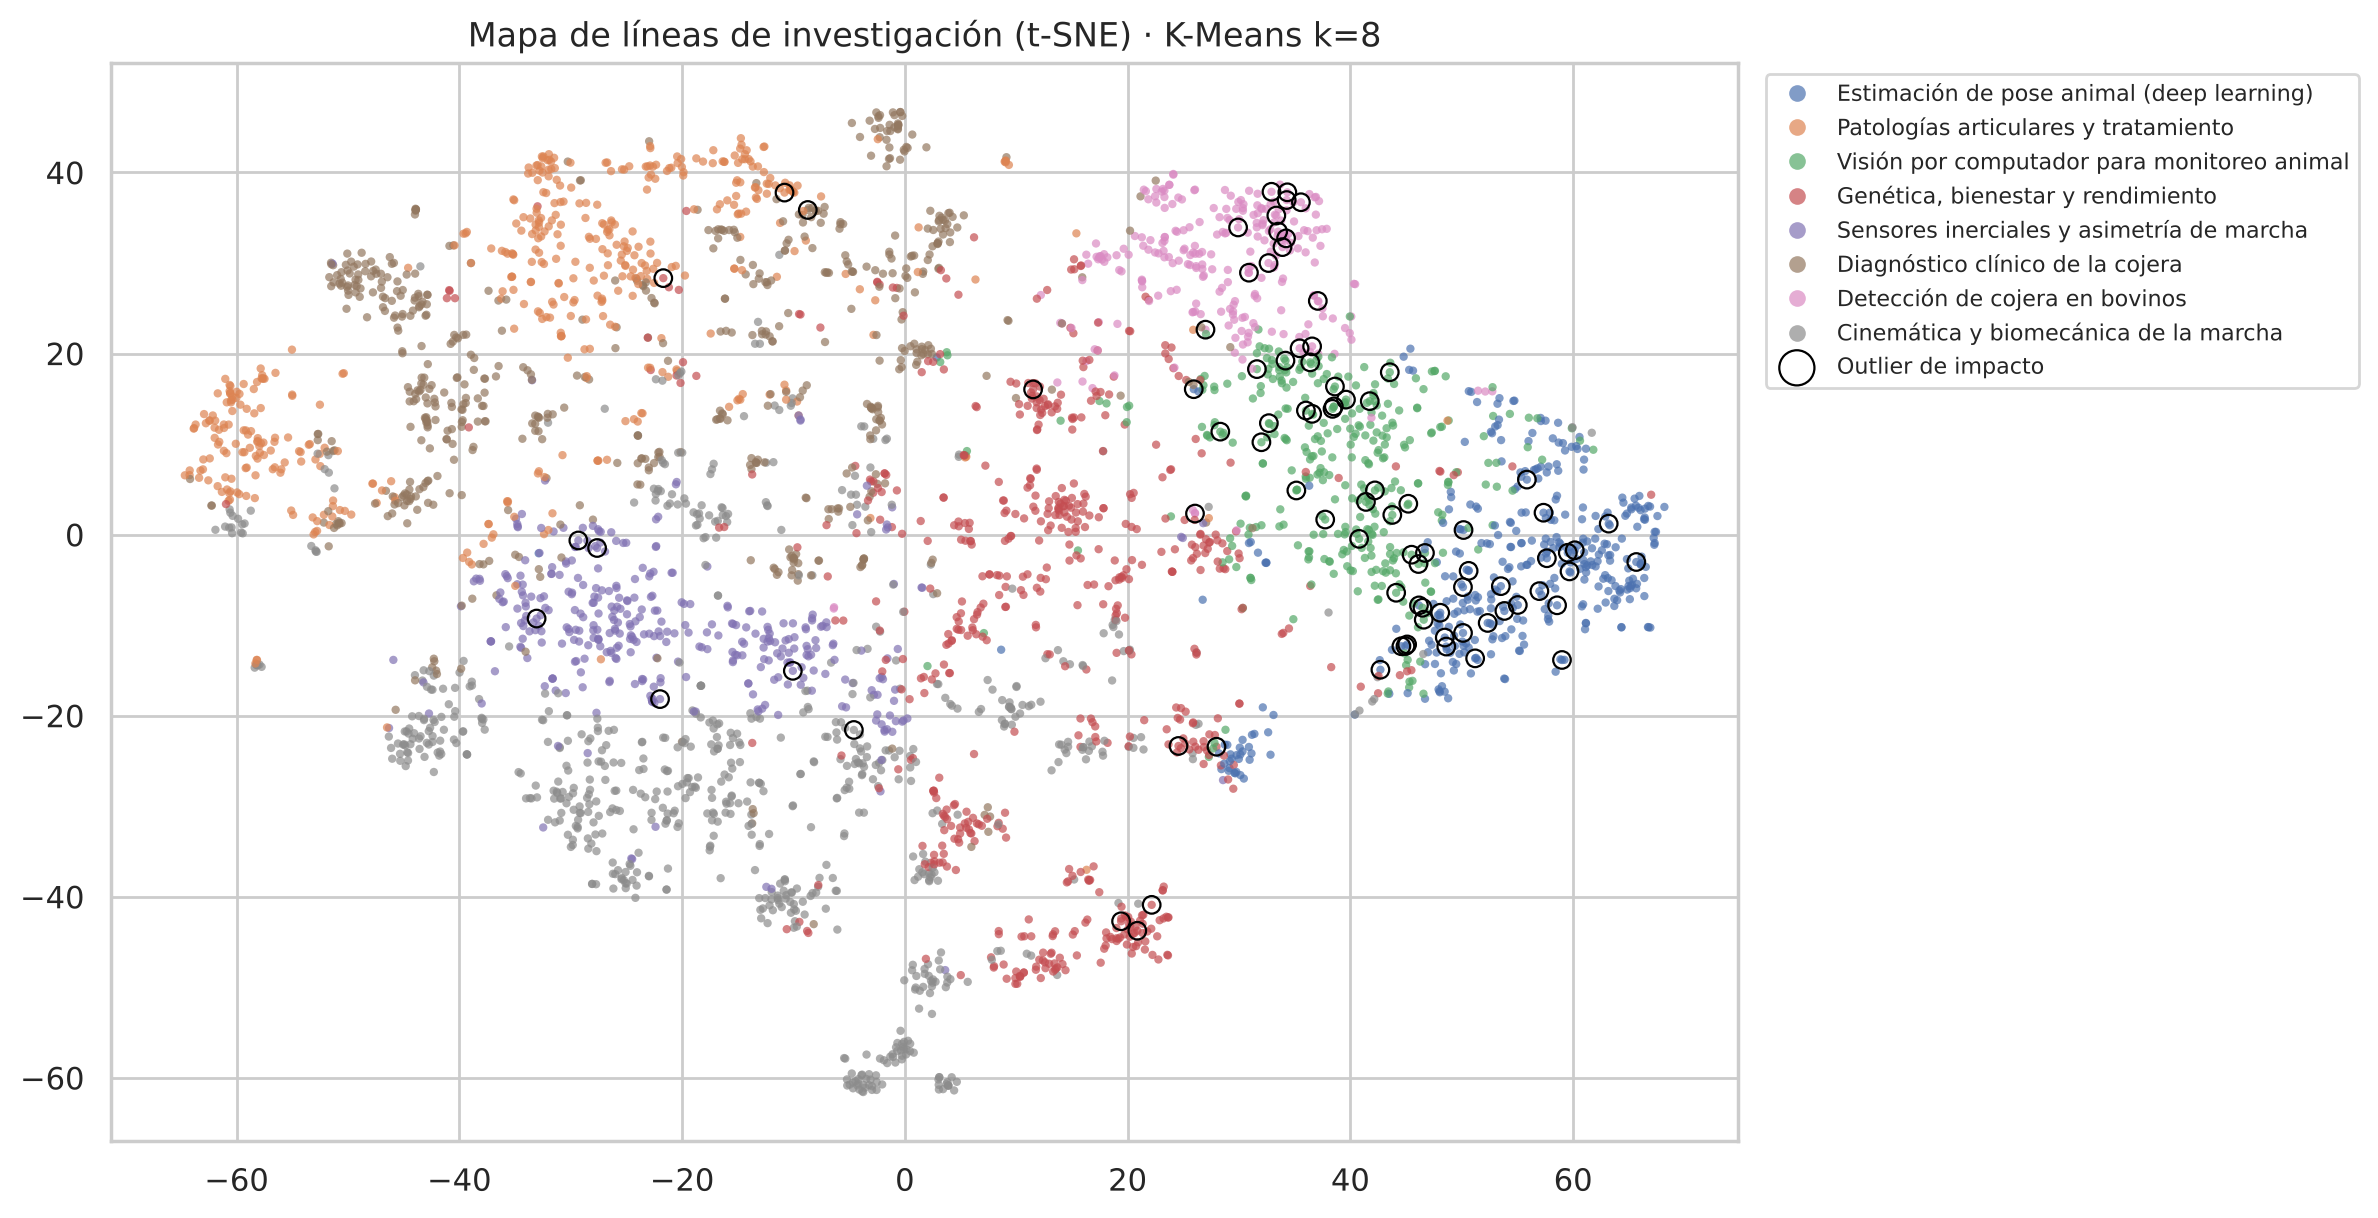
\includegraphics[width=\columnwidth]{art_tsne_clusters.png}
\caption{Mapa t-SNE de las líneas de investigación. Los círculos negros marcan los outliers de impacto, concentrados en los perfiles tecnológicos.}
\label{fig:tsne}
\end{figure}

\subsection{Perfiles de datasets públicos}
El clustering de Gower produce cuatro perfiles: (P1) video multivista con mocap 3D de caballos (PFERD, Zúrich), de alta precisión y pocos individuos; (P2) sensores IMU con etiqueta de cojera (caballo, vaca, oveja); (P3) imágenes estáticas de pose a gran escala (AP-10K, Animal-Pose, sintéticos); y (P4) video con keypoints (Horse-10, APT-36K, APTv2, Animal Kingdom, TigDog). De los 11 datasets que incluyen caballos, solo 2 tienen etiqueta de cojera y \textbf{ninguno combina video público con cojera}. La matriz de aptitud (Fig.~\ref{fig:aptitud}) ubica primero al dataset IMU usado aquí (0,77) y luego a Horse-10 (0,68) y PFERD (0,60). Esto define la estrategia para la fase final: preentrenar keypoints con AP-10K o Horse-10, validar las trayectorias contra el mocap de PFERD y aplicar el clasificador de simetría de este avance.

\begin{figure}[t]
\centering
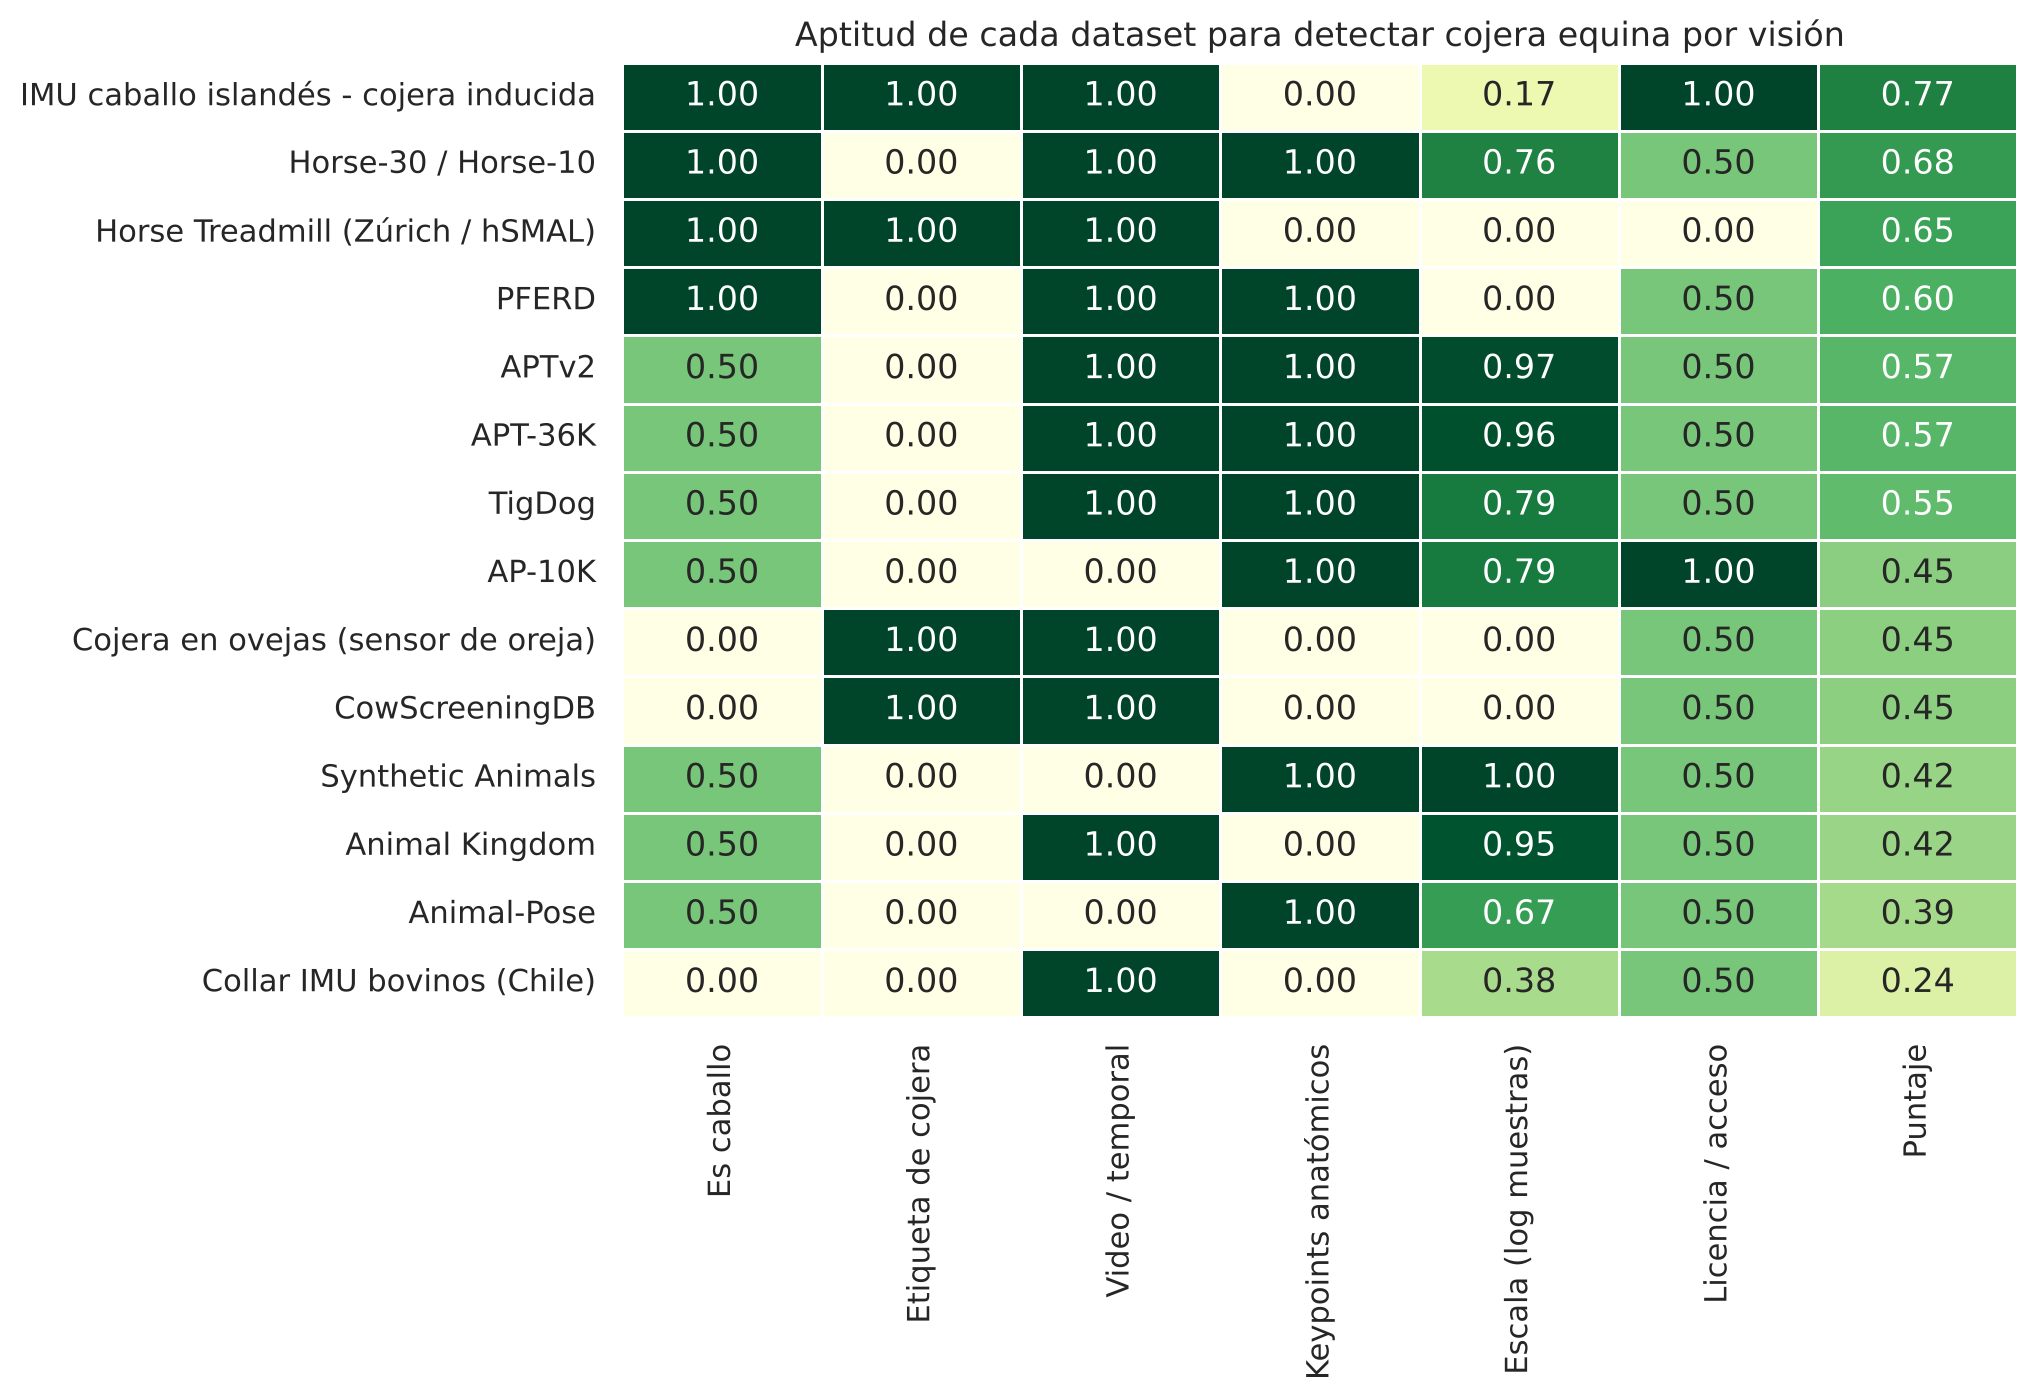
\includegraphics[width=0.92\columnwidth]{cat_matriz_aptitud.png}
\caption{Aptitud de cada dataset público para detectar cojera equina por visión (pesos: especie y etiqueta de cojera 0,25 cada uno; temporal y keypoints 0,15; escala y licencia 0,10).}
\label{fig:aptitud}
\end{figure}

\subsection{Señales de marcha: qué delata la cojera}
La Tabla~\ref{tab:wilcoxon} y la Fig.~\ref{fig:pareado} muestran que, con un análisis emparejado por caballo, la cojera anterior casi duplica la asimetría vertical de la cabeza (MinDiff +94\,\%, $p=0{,}004$) y reduce su \emph{harmonic ratio} ($-38$\,\%, $p=0{,}004$). La cojera posterior, en cambio, aumenta la asimetría del sacro (+53\,\%, $p=0{,}014$) y el \emph{hip hike} (+41\,\%, $p=0{,}042$). Es el patrón descrito en la clínica: el caballo levanta la cabeza al apoyar el miembro anterior doloroso, o la pelvis si el dolor está en el miembro posterior. La respuesta varía entre individuos: algunos casi no cambian. K-Means separó un perfil de zancadas de alta asimetría que agrupa el 36\,\% de las zancadas con cojera posterior y solo el 12\,\% de las sanas. El clustering jerárquico de caballo-condición formó un grupo mayoritariamente sano (15 de 20) y otro mayoritariamente cojo (10 de 13). Los grupos mixtos corresponden a caballos asimétricos de base, lo que indica que un umbral fijo no basta.

\begin{table}[t]
\centering
\caption{Cambio por inducción (medianas por caballo, Wilcoxon emparejado)}
\label{tab:wilcoxon}
\footnotesize\setlength{\tabcolsep}{3.5pt}
\begin{tabular}{llrrrr}
\toprule
Exp. & Variable & BAS & IND & $\Delta$\% & $p$ \\
\midrule
\multirow{3}{*}{Ant. ($n$=9)} & MinDiff cabeza (mm) & 16,2 & 31,4 & +94 & \textbf{0,004} \\
 & HR cabeza & 4,02 & 2,50 & $-38$ & \textbf{0,004} \\
 & MinDiff sacro (mm) & 8,9 & 8,0 & $-11$ & 1,000 \\
\midrule
\multirow{3}{*}{Post. ($n$=11)} & MinDiff sacro (mm) & 7,1 & 10,9 & +53 & \textbf{0,014} \\
 & \emph{Hip hike} (mm) & 12,5 & 17,6 & +41 & \textbf{0,042} \\
 & MinDiff cabeza (mm) & 17,0 & 17,8 & +4 & 0,577 \\
\bottomrule
\end{tabular}
\end{table}

\begin{figure}[t]
\centering
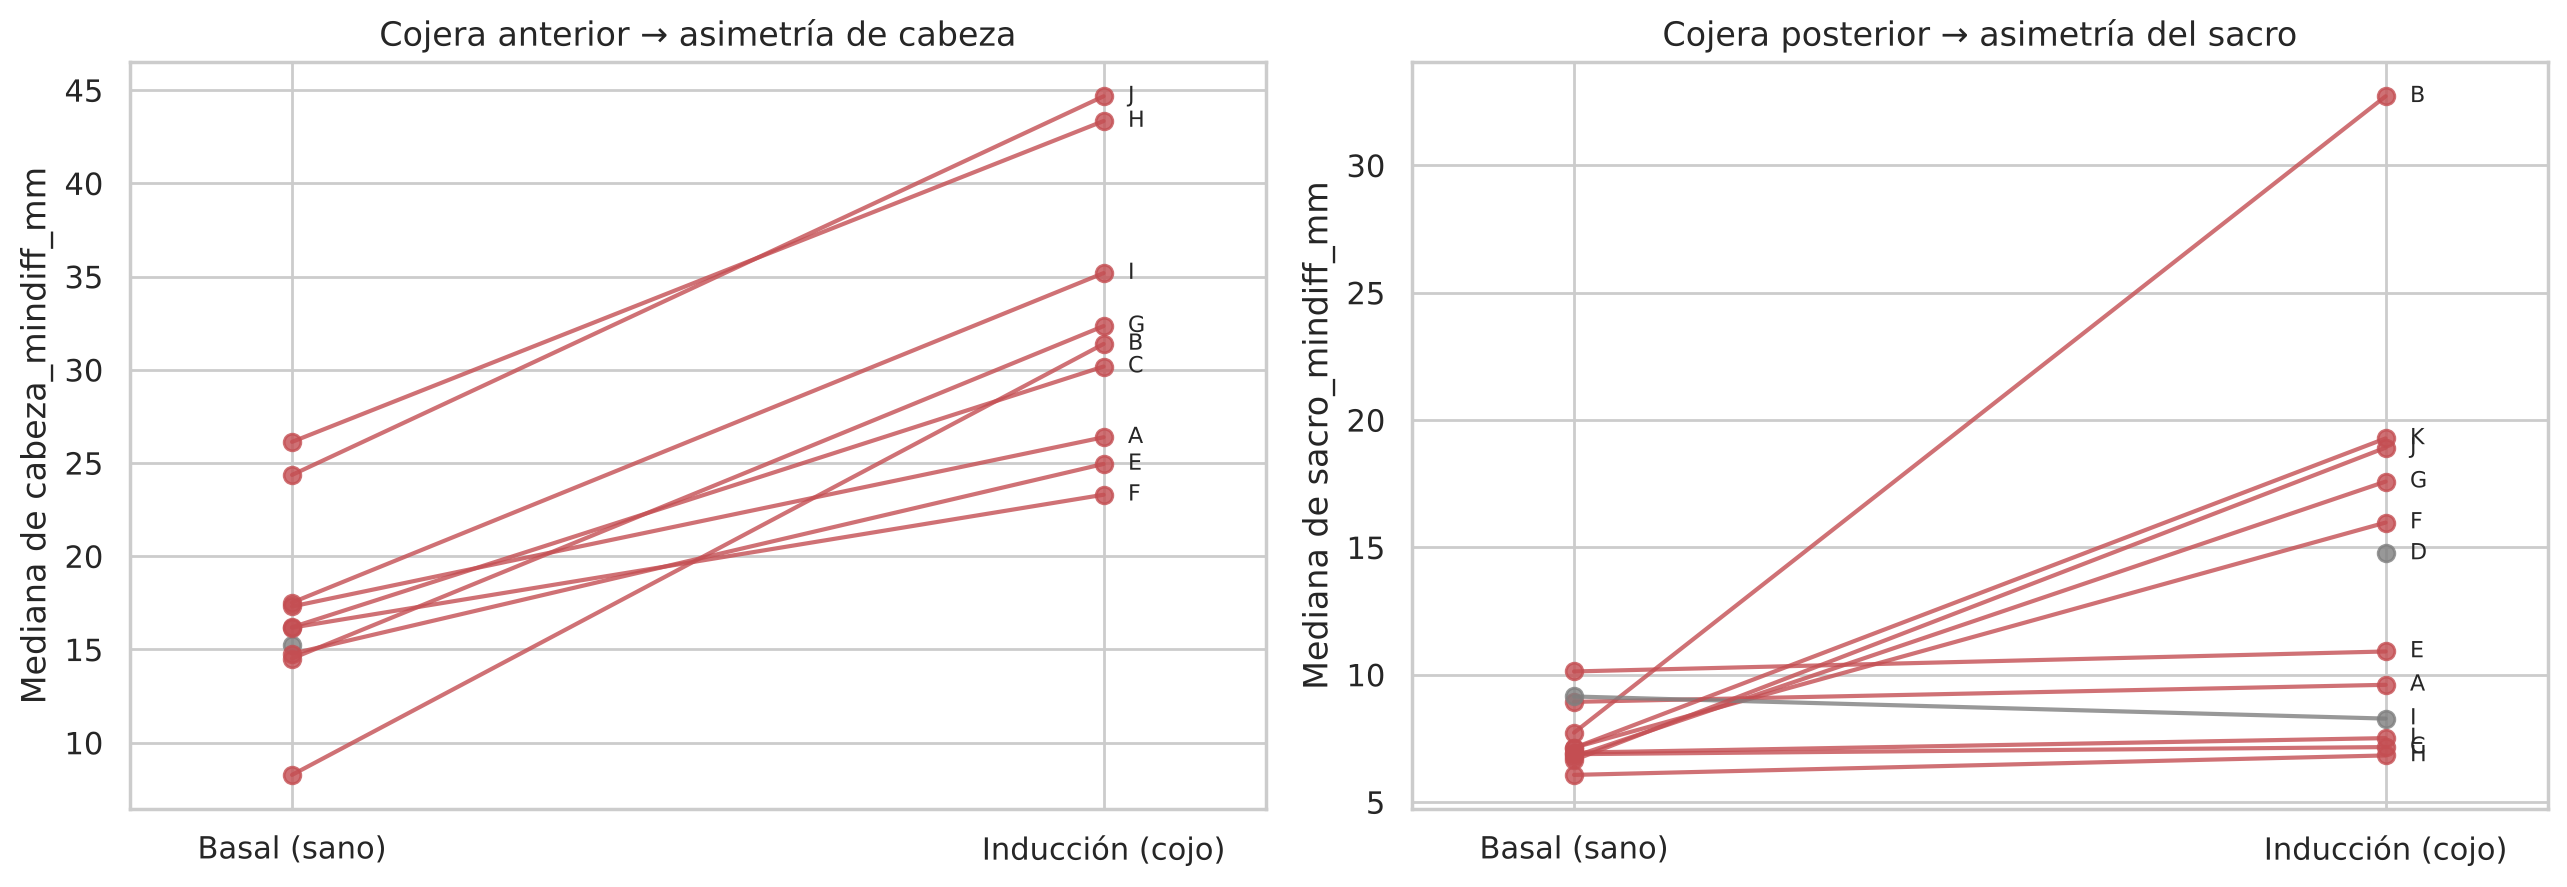
\includegraphics[width=\columnwidth]{imu_pareado_caballos.png}
\caption{Cambio individual de la mediana de asimetría entre la condición basal y la inducción. Cada línea es un caballo.}
\label{fig:pareado}
\end{figure}

\subsection{Modelo preliminar}
En validación cruzada agrupada, los modelos base y los ensembles quedaron en un rango estrecho de ROC-AUC (0,60--0,67, Tabla~\ref{tab:ml}). Tras la optimización, Random Forest (profundidad 8, 5 muestras por hoja, 200 árboles) fue el mejor ensemble en CV (0,666) y se eligió como modelo final, conforme al requisito de ensemble e interpretabilidad. En los 5 caballos de prueba obtuvo un ROC-AUC de \textbf{0,71}; en LOHO, también 0,71. Al promediar las zancadas de cada prueba de trote, clasificó bien 7 de 9 pruebas (Fig.~\ref{fig:roc}). Gradient Boosting rindió algo mejor en prueba (0,72), pero fue peor en CV, por lo que no se eligió para no sesgar la selección hacia el conjunto de prueba. SHAP (Fig.~\ref{fig:shap}) muestra que el modelo se apoya en MinDiff del sacro, el \emph{harmonic ratio} de la cabeza y la asimetría de la tuberosidad coxal: los mismos marcadores de la biomecánica. El rendimiento es moderado y honesto: la cojera inducida es leve y algunos caballos son asimétricos incluso sanos. Una partición aleatoria por zancada inflaría las métricas al permitir reconocer a cada caballo.

\begin{table}[t]
\centering
\caption{Resultados de clasificación (validación agrupada por caballo)}
\label{tab:ml}
\setlength{\tabcolsep}{3pt}
\begin{tabular}{lccc}
\toprule
Modelo & AUC CV (base) & AUC CV (optim.) & AUC prueba \\
\midrule
Regresión logística & 0,665 & --- & 0,684 \\
KNN ($k$=15) & 0,661 & --- & --- \\
SVM (RBF) & 0,665 & 0,677 & 0,690 \\
AdaBoost & 0,603 & --- & --- \\
Gradient Boosting & 0,611 & 0,634 & 0,721 \\
\textbf{Random Forest (final)} & 0,646 & \textbf{0,666} & \textbf{0,710} \\
\bottomrule
\end{tabular}
\end{table}

\begin{figure}[t]
\centering
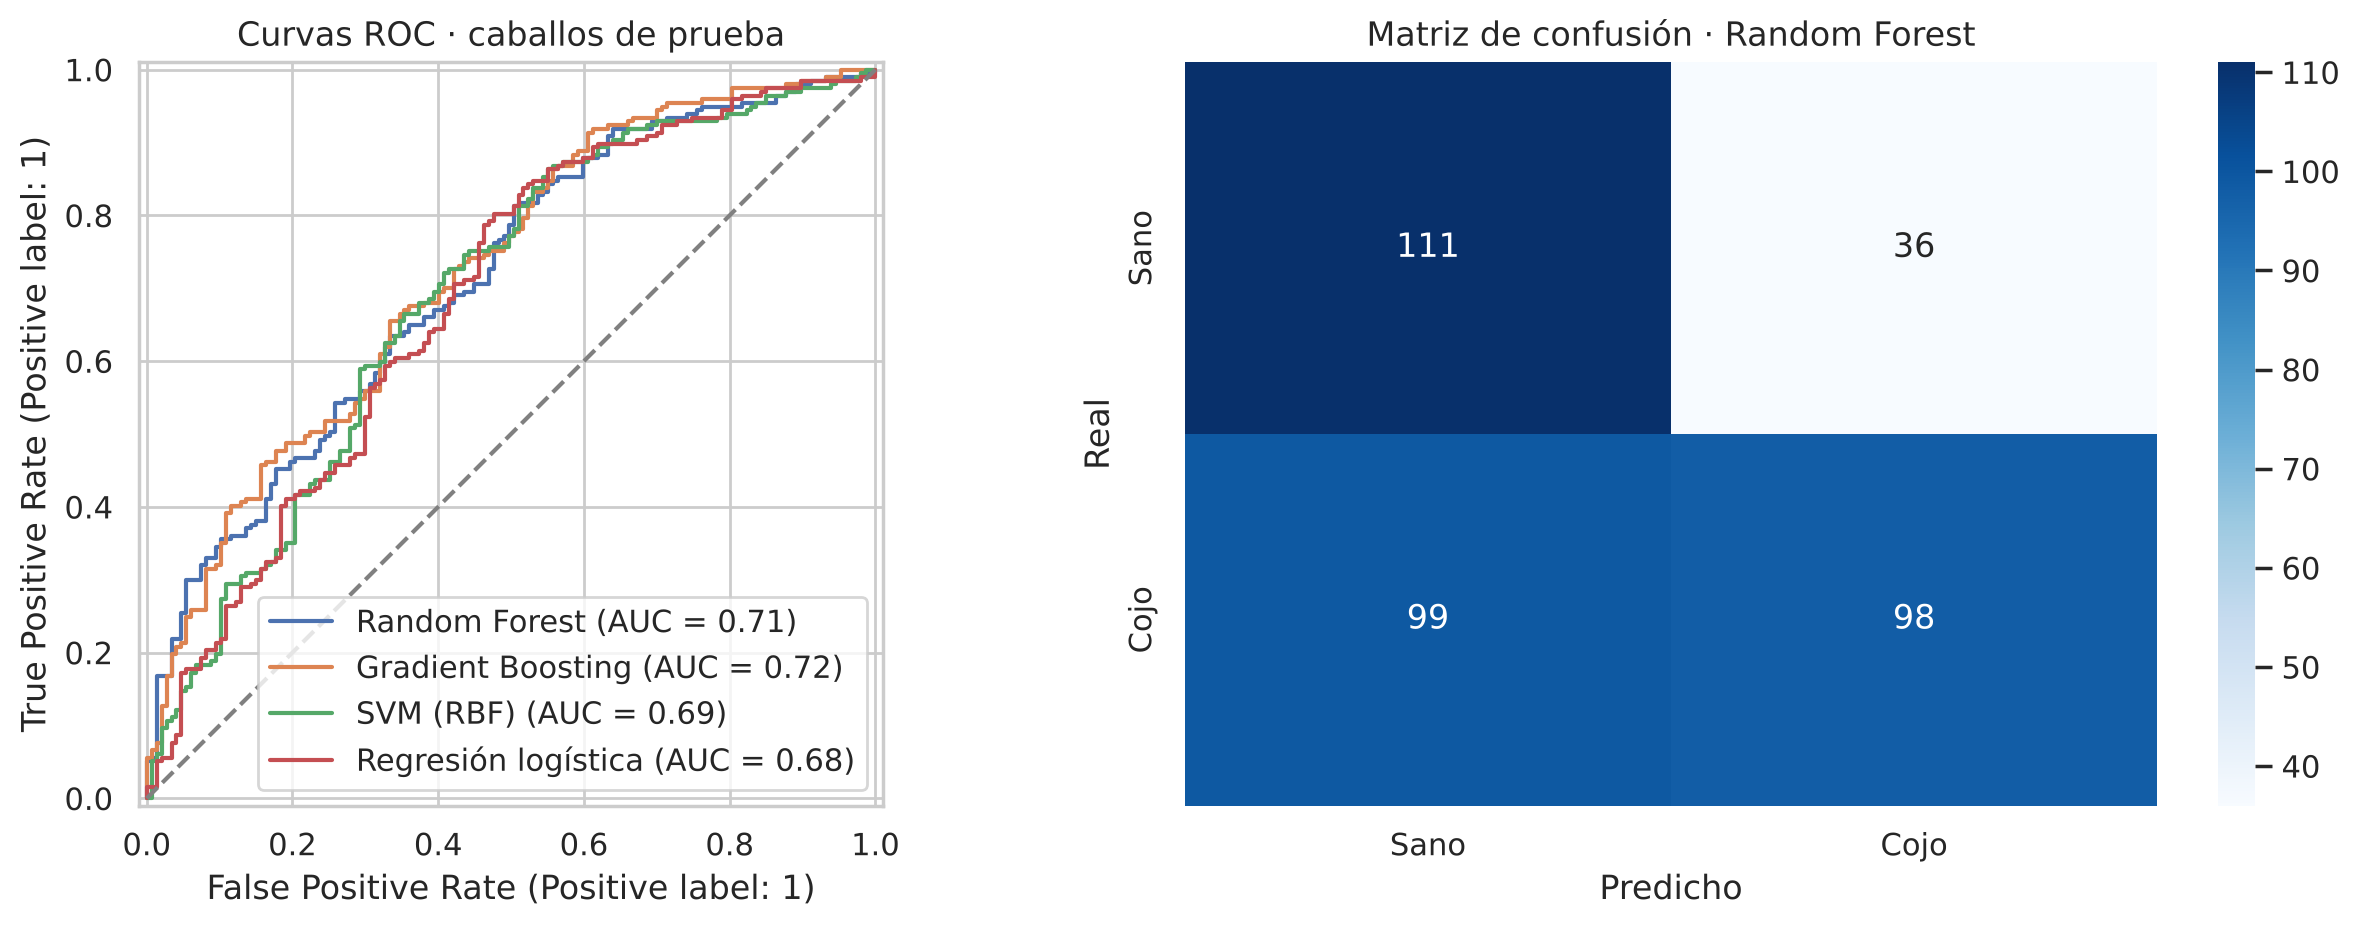
\includegraphics[width=\columnwidth]{ml_roc_confusion.png}
\caption{Curvas ROC en los 5 caballos de prueba y matriz de confusión del modelo final.}
\label{fig:roc}
\end{figure}

\begin{figure}[t]
\centering
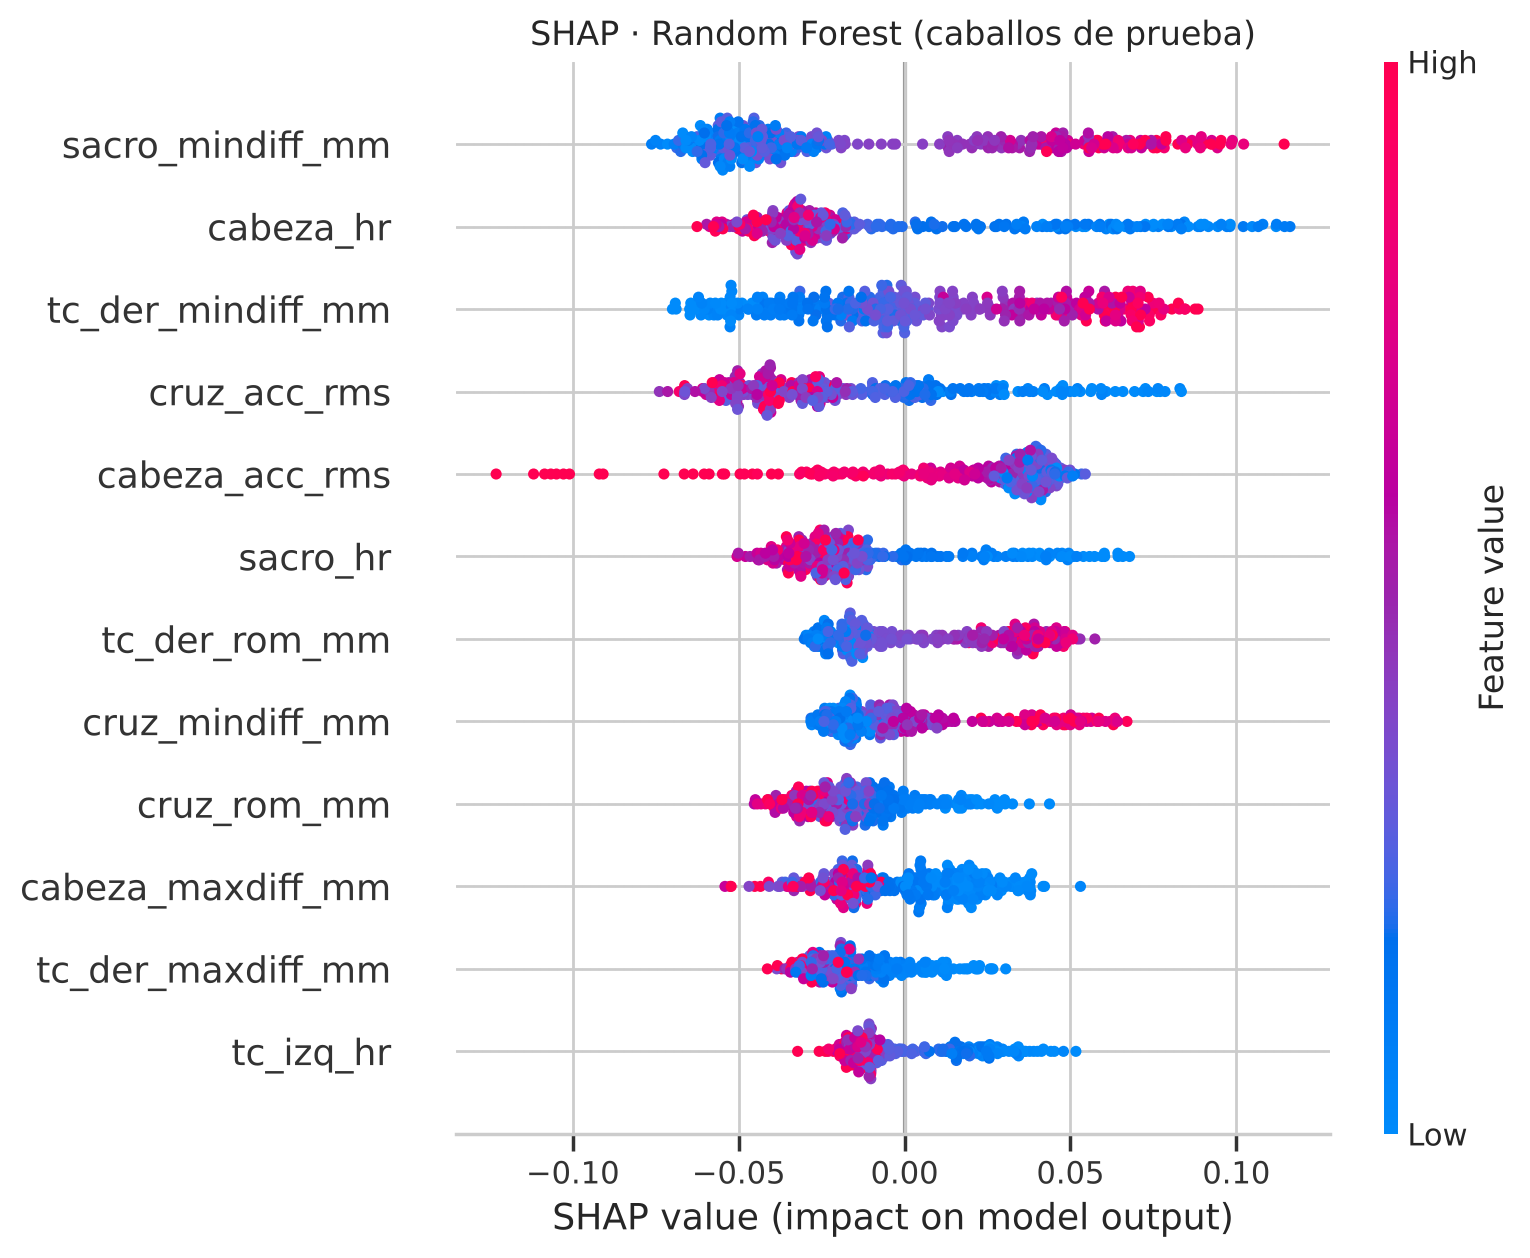
\includegraphics[width=0.85\columnwidth]{ml_shap_summary.png}
\caption{Valores SHAP del Random Forest: valores altos de asimetría (rojo) aumentan la probabilidad de cojera.}
\label{fig:shap}
\end{figure}

\subsection{Estimación preliminar de costos}
La Tabla~\ref{tab:costos} estima el costo mensual en us-east-1 con precios de lista on-demand: Lambda a USD 0,20 por millón de solicitudes y USD 0,0000166667 por GB-s (x86), API HTTP a USD 1,00 por millón y DynamoDB a USD 0,625 por millón de escrituras. El escenario académico cuesta USD 0,37 al mes (USD 0,13 con la capa gratuita): la base es prácticamente gratuita gracias al diseño serverless y a guardar la clave en Parameter Store en lugar de Secrets Manager. Un piloto con 50 clínicas, 20.000 pruebas al mes y réplica DR cuesta unos USD 13,5 al mes, dominado por el almacenamiento. Los costos \emph{reales} se medirán con Cost Explorer, filtrando por la etiqueta del proyecto, tras el despliegue de la entrega final.

\begin{table}[t]
\centering
\caption{Costo mensual estimado (USD, sin capa gratuita)}
\label{tab:costos}
\setlength{\tabcolsep}{4pt}
\begin{tabular}{lrr}
\toprule
Servicio & Académico & Piloto \\
\midrule
S3 (Standard, Glacier, PUT) & 0,17 & 6,90 \\
S3 réplica DR (Standard-IA + transferencia) & --- & 2,90 \\
Lambda (ingesta + inferencia) & 0,02 & 0,68 \\
API Gateway HTTP & 0,00 & 0,02 \\
DynamoDB (on-demand + PITR) & 0,01 & 0,46 \\
Athena & 0,03 & 1,00 \\
Parameter Store, ECR, CloudWatch & 0,15 & 1,55 \\
\midrule
\textbf{Total} & \textbf{0,37} & \textbf{13,51} \\
\bottomrule
\end{tabular}
\end{table}

% =====================================================================
\section{Plan de trabajo hacia la entrega final}
\begin{enumerate}
\item \textbf{ML:} normalizar cada caballo frente a una sesión de referencia propia (seguimiento longitudinal), calcular asimetrías con signo usando los sensores de casco, añadir modelos de regresión para estimar el grado de asimetría y aplicar LIME.
\item \textbf{Visión:} estimar keypoints de cabeza, cruz y pelvis desde video (preentrenamiento con AP-10K u Horse-10), validar contra PFERD y transferir el clasificador.
\item \textbf{Nube:} desplegar con \texttt{terraform apply}, publicar la API de inferencia, registrar los costos reales y preparar la demostración de extremo a extremo.
\item \textbf{Documento:} versión final en inglés y en español, y póster A1.
\end{enumerate}
\textbf{Riesgos:} pocos individuos (22 caballos), diferencia entre la cojera inducida y la natural, y sesgo racial del dataset (caballos islandeses). Se mitigarán con validación agrupada, reporte de la incertidumbre y validación externa futura con caballos criollos.

% =====================================================================
\section{Conclusiones}
La minería de datos de este avance cumple dos funciones. Mapea un campo que se desplaza con rapidez hacia la visión por computador, con un vacío claro de datos abiertos de video equino con cojera y de investigación latinoamericana. Además, valida con datos reales que las métricas de simetría vertical capturan la cojera de forma interpretable y coherente con la clínica. Este último resultado es el puente hacia la fase final: si la visión por computador estima esas mismas trayectorias desde un video, el clasificador y la arquitectura en la nube desarrollados aquí ya están listos para recibirlas. El código, los datos derivados y la infraestructura son reproducibles en el repositorio del proyecto.

\section*{Ética y datos}
Se usaron solo datos públicos con licencia abierta (OpenAlex CC0, dataset IMU CC BY 4.0). No se trataron datos personales. El protocolo experimental del dataset IMU es responsabilidad de sus autores, que lo publicaron con licencia abierta~\cite{smit2023dataset}. El sistema es una herramienta de apoyo y no reemplaza el examen veterinario.

\begin{thebibliography}{99}
\bibitem{agronegocios2025censo} Agronegocios, ``¿Cuántos caballos hay en Colombia y de esta cifra cuántos están registrados?,'' \emph{Agronegocios}, 2025. [En línea]. Disponible: \url{https://www.agronegocios.co/finca/cuantos-caballos-hay-en-colombia-y-de-esta-cifra-cuantos-estan-registrados-4206155}
\bibitem{nehs2013} ``Equine health survey highlights the prevalence of lameness,'' \emph{Veterinary Record}, vol.~173, no.~6, p.~132, 2013, doi: 10.1136/vr.f4967.
\bibitem{usda1998} USDA APHIS, ``National economic cost of equine lameness, colic, and equine protozoal myeloencephalitis (EPM) in the United States,'' Info sheet, NAHMS Equine'98, Fort Collins, CO, EE.~UU.
\bibitem{keegan2010} K.~G. Keegan \emph{et al.}, ``Repeatability of subjective evaluation of lameness in horses,'' \emph{Equine Vet. J.}, vol.~42, no.~2, pp.~92--97, 2010, doi: 10.2746/042516409X479568.
\bibitem{hammarberg2016} M.~Hammarberg, A.~Egenvall, T.~Pfau y M.~Rhodin, ``Rater agreement of visual lameness assessment in horses during lungeing,'' \emph{Equine Vet. J.}, vol.~48, no.~1, pp.~78--82, 2016, doi: 10.1111/evj.12385.
\bibitem{un2015} Naciones Unidas, ``Transformar nuestro mundo: la Agenda 2030 para el Desarrollo Sostenible,'' Res. A/RES/70/1, 2015.
\bibitem{keegan2013} K.~G. Keegan \emph{et al.}, ``Comparison of a body-mounted inertial sensor system-based method with subjective evaluation for detection of lameness in horses,'' \emph{Am. J. Vet. Res.}, vol.~74, no.~1, pp.~17--24, 2013.
\bibitem{mathis2018} A.~Mathis \emph{et al.}, ``DeepLabCut: markerless pose estimation of user-defined body parts with deep learning,'' \emph{Nature Neuroscience}, vol.~21, pp.~1281--1289, 2018, doi: 10.1038/s41593-018-0209-y.
\bibitem{mathis2021} A.~Mathis \emph{et al.}, ``Pretraining boosts out-of-domain robustness for pose estimation,'' en \emph{Proc. IEEE/CVF WACV}, 2021, pp.~1859--1868.
\bibitem{li2024pferd} C.~Li \emph{et al.}, ``The Poses for Equine Research Dataset (PFERD),'' \emph{Scientific Data}, vol.~11, art.~497, 2024, doi: 10.1038/s41597-024-03312-1.
\bibitem{yu2021ap10k} H.~Yu, Y.~Xu, J.~Zhang, W.~Zhao, Z.~Guan y D.~Tao, ``AP-10K: A benchmark for animal pose estimation in the wild,'' en \emph{NeurIPS Datasets and Benchmarks Track}, 2021.
\bibitem{yang2022apt36k} Y.~Yang, J.~Yang, Y.~Xu, J.~Zhang, L.~Lan y D.~Tao, ``APT-36K: A large-scale benchmark for animal pose estimation and tracking,'' en \emph{NeurIPS Datasets and Benchmarks Track}, 2022.
\bibitem{ng2022animalkingdom} X.~L. Ng, K.~E. Ong, Q.~Zheng, Y.~Ni, S.~Y. Yeo y J.~Liu, ``Animal Kingdom: A large and diverse dataset for animal behavior understanding,'' en \emph{Proc. IEEE/CVF CVPR}, 2022, pp.~19023--19034.
\bibitem{ismail2024cow} S.~Ismail, M.~Diaz, C.~Carmona-Duarte, J.~M. Vilar y M.~A. Ferrer, ``CowScreeningDB: A public benchmark database for lameness detection in dairy cows,'' \emph{Comput. Electron. Agric.}, vol.~216, art.~108500, 2024.
\bibitem{priem2022openalex} J.~Priem, H.~Piwowar y R.~Orr, ``OpenAlex: A fully-open index of scholarly works, authors, venues, institutions, and concepts,'' arXiv:2205.01833, 2022.
\bibitem{smit2023dataset} I.~Smit \emph{et al.}, ``Kinematic data of the Icelandic horse with induced lameness at walk, trot and tölt,'' DataverseNL, 2025, doi: 10.34894/PEWAK6.
\bibitem{iglewicz1993} B.~Iglewicz y D.~C. Hoaglin, \emph{How to Detect and Handle Outliers}. Milwaukee, WI, EE.~UU.: ASQC Quality Press, 1993.
\bibitem{lundberg2017} S.~M. Lundberg y S.-I. Lee, ``A unified approach to interpreting model predictions,'' en \emph{Advances in Neural Information Processing Systems 30}, 2017, pp.~4765--4774.
\bibitem{wirth2000} R.~Wirth y J.~Hipp, ``CRISP-DM: Towards a standard process model for data mining,'' en \emph{Proc. 4th Int. Conf. Practical Applications of Knowledge Discovery and Data Mining}, 2000, pp.~29--39.
\end{thebibliography}

\end{document}
